%%%%%%%%%%%%%%%%%%%%%%%%%%%%%%%%%%%%
% Header                           %
%%%%%%%%%%%%%%%%%%%%%%%%%%%%%%%%%%%%
% 
% Revisions: 2017-04-10 Martin R�del <martin.raedel@dlr.de>
%                       Initial draft
%               
% Contact:   Martin R�del,  martin.raedel@dlr.de
%            DLR Composite Structures and Adaptive Systems
%          
%                                 __/|__
%                                /_/_/_/  
%            www.dlr.de/fa/en      |/ DLR
% 
%%%%%%%%%%%%%%%%%%%%%%%%%%%%%%%%%%%%
% Content                          %
%%%%%%%%%%%%%%%%%%%%%%%%%%%%%%%%%%%%

\levelup{Preferences}

\leveldown{Change mesh on sphere \texttt{Glyph}}

Sometimes for nice publication pictures the default sphere glyph representation might be a little too angular. Internally, sphere glyphs are nothing but a combination of a certain number of tetrahedron elements. Thus, the mesh behind a sphere glyph might be too coarse. It is assumed you already have a glyph as spheres, otherwise have a look at \autoref{sec:ParaView_Damage_Plots_on_Nodes_as_Spheres}. 

In order to change the mesh size and smooth the sphere shape perform the following steps:

\begin{enumerate}[noitemsep]
\item Select the Glyph in the \textit{Pipeline Browser}
\item In the \textit{Properties} tab
  \begin{itemize}[noitemsep]
  \item Below the top line press the gear symbol 
\includegraphics[width=\iconsize]{Figures/Icons/pqAdvanced26}
  \item Additional options in section \textit{Glyph Source} appear
  \item Adjust the values for \textit{Theta resolution} and \textit{Phi resolution} to your needs. The default coarse value is 8.
  \item Click 
\includegraphics[width=\iconsize]{Figures/Icons/pqAutoApply32} \textit{Apply}
  \end{itemize}
\end{enumerate}

The result is compared in \autoref{fig:ParaView_Glyph_Mesh}. The mesh refinement has a significant impact on the computational performance. So only use the refined mesh if it is really necessary.

\begin{figure}[htbp]
  \begin{subfigure}{0.49\linewidth}
    \centering
    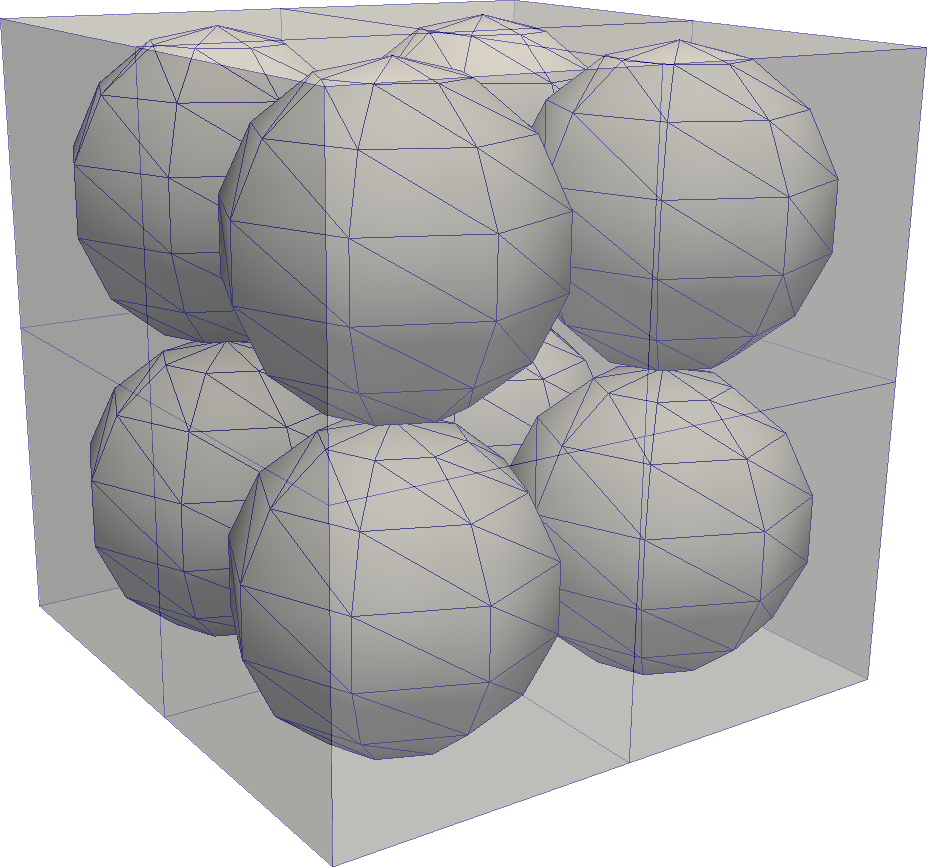
\includegraphics[width=0.85\linewidth]{Figures/ParaView/ParaView_Glyph_Mesh8}
    \caption{Resolution=8}
    \label{fig:ParaView_Glyph_Mesh8}
  \end{subfigure}%
  \begin{subfigure}{0.49\linewidth}
    \centering
    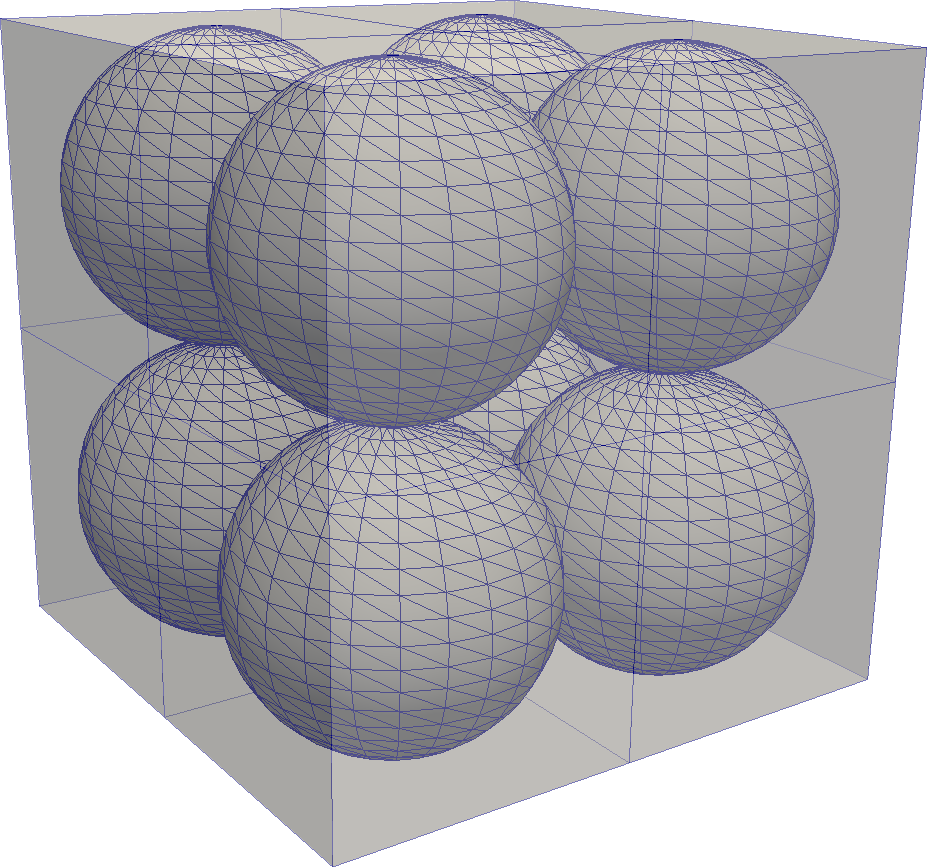
\includegraphics[width=0.85\linewidth]{Figures/ParaView/ParaView_Glyph_Mesh24}
    \caption{Resolution=24}
    \label{fig:ParaView_Glyph_Mesh24}
  \end{subfigure}%
  \caption{\protect\marktool{\toolname} collocation points inside the base finite element mesh with different glyph resolutions}
  \label{fig:ParaView_Glyph_Mesh}
\end{figure}

